\documentclass[12pt]{article}
\usepackage{signals-style}   % shared style: styles/signals-style.sty

\begin{document}

\tutorialpage{01}{September 2026}

\begin{enumerate}

% ---------------- Q2 ----------------
\item Sketch the following signals.
\begin{multicols}{2}
\begin{enumerate}
    \item $x(t)=\sin (2\pi t)$
    \item $x(t)=\cos (\pi t/4)$
    \item $x(t)=\sin (\pi t/2 - \pi/6)$
    \item $x(t) = u(t-5)$
    \item $x(t) = e^{-t}u(t)$
    \item $x[n] = \sin(\pi n /6)$
\end{enumerate}
\end{multicols}


% ---------------- Q1 ----------------
\item A continuous time signal is given in Figure \ref{fig:q1}. Sketch and label the following signals. \\
\begin{enumerate*}
    \item $x(t)+1$ \item $2x(t)-1$ \item $-x(t)$ \item $-2x(t)+1$ \item $x(t-1)$ \item $x(-t)$ \item $x(-t + 1)$ \item $x(2t)$ \item $x(t/2 + 1)$
\end{enumerate*}

\begin{center}
\begin{tikzpicture}
    \begin{axis}[
    width = 7cm,
    height = 4cm,
    axis lines = left,
    xlabel = $t$,
    ylabel = $x(t)$,
    xmin = 0, xmax = 3.5,
    ymin = 0, ymax = 1.5,
    samples = 200,
    xtick distance = 1,
    ytick distance = 1,
    xlabel style={
        at={(axis description cs:1.05,0.2)},
        anchor=west
    },
    ylabel style={
        at={(axis description cs:0.23,1)},
        anchor=south,
        rotate=-90
    },
    grid = both
    ]

    \addplot[domain=0:1, thick]{x};
    \addplot[domain=1:2, thick]{1};
    \addplot[thick]coordinates{(2,0) (2,1)};
    \addplot[domain=2:3, thick]{0};
    \end{axis}
\end{tikzpicture}
\captionof{figure}{}
\label{fig:q1}
\end{center}

% ---------------- Q2 ----------------
\item A discrete time signal is shown in Figure \ref{fig:q2}. Sketch and label each of the following signals.
\begin{enumerate*}
    \item $2x[n] - 1$ \item $-x[n] + 1$ \item $x[n+1]$ \item $x[-n+2]$ \item $x[2n+1]$ \item $$x[n/2]$$
\end{enumerate*}

\begin{center}
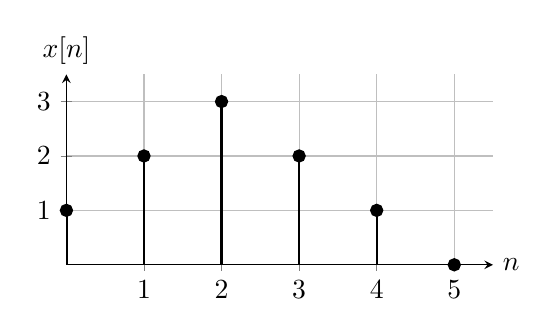
\begin{tikzpicture}
    \begin{axis}[
        width=7cm,
        height=4cm,
        axis lines=middle,
        xmin=0, xmax=5.5,
        ymin=0, ymax=3.5,
        xtick={0,1,2,3,4,5},
        ytick={0,1,2,3},
        xlabel={$n$},
        ylabel={$x[n]$},
        xlabel style={
            at={(axis description cs:1,0)},
            anchor=west
        },
        ylabel style={
            at={(axis description cs:0,1)},
            anchor=south,
            rotate=0
        },
        grid = both
    ]

    \addplot[
        ycomb,
        mark=*,
        thick
    ] coordinates {
        (0,1)
        (1,2)
        (2,3)
        (3,2)
        (4,1)
        (5,0)
    };

    \end{axis}
\end{tikzpicture}
\captionof{figure}{}
\label{fig:q2}
\end{center}

% ---------------- Q4----------------
\item Determine whether or not the following signals are periodic. If periodic, determine the period of the signal.
\begin{enumerate}
    \item $x(t)=\sin (\pi t)$
    \item $x(t)=\sin (\pi t + \pi/4)$
    \item $x(t)=e^t \sin (\pi t /4)$
    \item $x[n]=\sin(\pi n/4)$
    \item $x[n]=\sin(2n)$
\end{enumerate}


% ---------------- Q4----------------
\item Determine the following signals to be odd, even or neither. (Use both definition of an odd/even signal and graphing to determine.)
\begin{enumerate}
    \item $x(t)=\sin (\pi t)$
    \item $x(t)=\cos (\pi t)$
    \item $x(t)=\sin (\pi t + \pi/4)$
\end{enumerate}

% ---------------- Q5----------------
\item It can be shown that any real signal can be decomposed into an odd signal and an even signal using the following formulas.
\[x(t)=x_e(t)+x_o(t)\]
where;
\[x_e(t)=\frac{x(t)+x(-t)}{2}\]
\[x_o(t)=\frac{x(t)-x(-t)}{2}\].
Find and sketch the odd and even signals of the signal represented in Figure \ref{fig:q1}.

% ---------------- Q6 ----------------
\item Show that
\[
\int_{-a}^{a} x(t)\,dt =
\begin{cases}
2\displaystyle\int_{0}^{a} x(t)\,dt, & \text{if } x(t) \text{ is even}, \\[1em]
0, & \text{if } x(t) \text{ is odd}.
\end{cases}
\]

% ---------------- Q7 ----------------
\item Show that the complex exponential signal $x(t) = \ejw{\omega t}$ is periodic and that its fundamental period is $2\pi/\omega$.

\begin{keyresult}
$T_0 = 2\pi/\omega$ is the smallest positive $T$ satisfying $\ejw{\omega(t+T)} = \ejw{\omega t}$.
\end{keyresult}

% ---------------- Q8 ----------------
\item Show that the complex exponential signal $x[n] = \ejw{\omega n}$ is periodic only if $\omega/2\pi$ is a rational number.

% ---------------- Q19 ----------------
\item Determine whether the following signals are energy signals, power signals, or neither.
\begin{enumerate}
    \item $x(t) = e^{-at}\,u(t), \; a>0$
    \item $x(t) = A\cos(\omega t + \theta)$
    \item $x[n] = 3\,u[n]$
    \item $x[n] = 3e^{3n}$
\end{enumerate}

\end{enumerate}

\end{document}
